% Template LaTeX file for DAFx-08 papers % (fold)
%
% To generate the correct references using BibTeX, run
%     latex, bibtex, latex, latex
% modified...
% - from DAFx-00 to DAFx-02 by Florian Keiler, 2002-07-08
% - from DAFx-02 to DAFx-03 by Gianpaolo Evangelista
% - from DAFx-05 to DAFx-06 by Vincent Verfaille, 2006-02-05
% - from DAFx-06 to DAFx-07 by Vincent Verfaille, 2007-01-05
%                          and Sylvain Marchand, 2007-01-31
% - from DAFx-07 to DAFx-08 by Henri Penttinen, 2007-12-12
%                          and Jyri Pakarinen 2008-01-28
%
% Template with hyper-references (links) active after conversion to pdf
% (with the distiller) or if compiled with pdflatex.
%
% 20060205: added package 'hypcap' to correct hyperlinks to figures and tables
%                      use of \papertitle and \paperauthorA, etc for same title in PDF and Metadata
%
% 1) Please compile using latex or pdflatex.
% 2) If using pdflatex, you need your figures in a file format other than eps! e.g. png or jpg is working
% 3) Please use "paperftitle" and "pdfauthor" definitions below


%%%%%%%%%%%%%%%%%%%%%%%%%%%%%%%%%%%%%%%%%%%%%%%%%%%%%%%%%%%%%%%%%%%%%
%%%%%%%%%%%%%%%%%%%%%%%%%%%%%%%%%%%%%%%%%%%%%%%%%%%%%%%%%%%%%%%%%%%%%
%%%%%%%%%%%%%%%%%%%%%%%%%%%%%%%%%%%%%%%%%%%%%%%%%%%%%%%%%%%%%%%%%%%%%
% 
% TTBlue Notes / Paper
% from conversation with Dave over coffee at Pre en Bulle in Albi
% 20 June 2008
% 
% 
% TTBlue is different from existing DSP libraries (such as Perry Cook's STK) in a number of ways:
% * Dynamic environment which itself can be queried for available components (using the TTFactory registry)
% * Dynamic binding, message passing architecture (reflective programming)
% 
% 
% Different from other C++ libraries in that it provides reflective programming techniques.
% Different from other languages with similar features in that it is implemented in C++ with good support for multiple platforms including embedded processor.
%  IEC 61508
%  Isograph
% 
% 
% Allows for:
% * programmatic creation of user interfaces
% * adaptive wrappers for various plug-in architectures (VST, AU, Max/MSP, SuperCollider)
% * dynamic, self-modifying networks of components 
% 
% 
% 
% 
% Try to see what we can learn from:
% * SuperCollider spawning thing for granular synthesis?
%  
% 
% 
% 
% Dynamic re-configuration of the signal networks and control structures means that TTBlue can be run on a web server and the signal chain defined (or re-defined) in real time on a web client using a GUI (such as a web browser or iPhone) or SMS.
% 
% One application of this is an installation or sculptural art work where you could tweak the behavior by sending it SMS messages using a phone.


% I would also like to develop a systematic approach for dealing with interpolation algorithms...
% Some sort of an interpolation library in TTBlue
% For example, this would allow us to apply the cubic interpolation everywhere without re-writing the code


%%%%%%%%%%%%%%%%%%%%%%%%%%%%%%%%%%%%%%%%%%%%%%%%%%%%%%%%%%%%%%%%%%%%%
%%%%%%%%%%%%%%%%%%%%%%%%%%%%%%%%%%%%%%%%%%%%%%%%%%%%%%%%%%%%%%%%%%%%%
%%%%%%%%%%%%%%%%%%%%%%%%%%%%%%%%%%%%%%%%%%%%%%%%%%%%%%%%%%%%%%%%%%%%%




%------------------------------------------------------------------------------------------
%  !  !  !  !  !  !  !  !  !  !  !  ! user defined variables  !  !  !  !  !  !  !  !  !  !  !  !  !  !
% Please use these commands to define title and author of the paper:
\def\papertitle{The Jamoma Multicore Audio Graph Layer}
\def\paperauthorA{Timothy Place?}
\def\paperauthorB{Trond Lossius?}
\def\paperauthorC{Nils Peters?}
\def\paperauthorD{Anyone Else?}


%------------------------------------------------------------------------------------------
\documentclass[twoside,a4paper]{article}
\usepackage{dafx_08}
\usepackage{amsmath,amssymb,amsfonts,amsthm}
\usepackage{subfigure,color}
\usepackage{euscript}
\usepackage[latin1]{inputenc}
\usepackage[T1]{fontenc}
\setcounter{page}{1}
\ninept

\usepackage{times}
% Saves a lot of ouptut space in PDF... after conversion with the distiller
% Delete if you cannot get PS fonts working on your system.

% pdf-tex settings: detect automatically if run by latex or pdflatex
\newif\ifpdf
\ifx\pdfoutput\relax
\else
   \ifcase\pdfoutput
      \pdffalse
   \else
      \pdftrue
\fi

\ifpdf % compiling with pdflatex
  \usepackage[pdftex,
    pdftitle={\papertitle},
    pdfauthor={\paperauthorA, \paperauthorB, \paperauthorC, \paperauthorD},
    colorlinks=false, % links are activated as colror boxes instead of color text
    bookmarksnumbered, % use section numbers with bookmarks
    pdfstartview=XYZ % start with zoom=100% instead of full screen; especially useful if working with a big screen :-)
  ]{hyperref}
  \pdfcompresslevel=9
  \usepackage[pdftex]{graphicx}
  \usepackage[figure,table]{hypcap}
\else % compiling with latex
  \usepackage[dvips]{epsfig,graphicx}
  \usepackage[dvips,
    colorlinks=false, % no color links
    bookmarksnumbered, % use section numbers with bookmarks
    pdfstartview=XYZ % start with zoom=100% instead of full screen
  ]{hyperref}
  % hyperrefs are active in the pdf file after conversion
  \usepackage[figure,table]{hypcap}
\fi

\title{\papertitle}

%-------------SINGLE-AUTHOR HEADER STARTS (uncomment below if your paper has a single author)-----------------------
%\affiliation{\paperauthorA}    % This command replaces \name{The DAFx Crew}
%{\href{http://www.acoustics.hut.fi/dafx08/}{Dept. of Signal Processing and Acoustics,} \\ Helsinki University of Technology, TKK \\ Espoo, Finland\\
%{\tt \href{mailto:dafx-08@acoustics.hut.fi}{dafx-08@acoustics.hut.fi}}}
%-----------------------------------SINGLE-AUTHOR HEADER ENDS------------------------------------------------------

%---------------TWO-AUTHOR HEADER STARTS (uncomment below if your paper has two authors)-----------------------
%\twoaffiliations{\paperauthorA, \sthanks{This work was supported by the XYZ Foundation}}
%{\href{
%http://www.acoustics.hut.fi/dafx08/}{Dept. of Signal Processing and Acoustics,} \\ Helsinki University of Technology, TKK \\ Espoo, Finland\\
%{\tt \href{mailto:dafx-08@acoustics.hut.fi}{dafx-08@acoustics.hut.fi}}
%}
%{\paperauthorB,\sthanks{This guy is a very good fellow}}
%{\href{http://www.acoustics.hut.fi/dafx08/}{Reading Group, Dept.~of Reading Sciences} \\ Univ.~of Universe, Sun \\ {\tt \href{mailto:dafx-08@acoustics.hut.fi}{dafx-08@acoustics.hut.fi}}
%}
%-------------------------------------TWO-AUTHOR HEADER ENDS------------------------------------------------------

%---------------THREE-AUTHOR HEADER STARTS (uncomment below if your paper has three authors)-----------------------
%\threeaffiliations{\paperauthorA, \sthanks{This work was supported by the XYZ Foundation}}
%{\href{
%http://www.acoustics.hut.fi/dafx08/}{Dept. of Signal Processing and Acoustics,} \\ Helsinki University of Technology, TKK \\ Espoo, Finland\\
%{\tt \href{mailto:dafx-08@acoustics.hut.fi}{dafx-08@acoustics.hut.fi}}
%}
%{\paperauthorB,\sthanks{This guy is a very good fellow}}
%{\href{http://www.acoustics.hut.fi/dafx08/}{Reading Group, Dept.~of Reading Sciences} \\ Univ.~of Universe, Sun \\ {\tt \href{mailto:dafx-08@acoustics.hut.fi}{dafx-08@acoustics.hut.fi}}
%}
%{\paperauthorC,\sthanks{She is a member of the Wheel Association}}
%{\href{http://www.acoustics.hut.fi/dafx08/}{Spinning Group, Dept.~of Turning Sciences} \\ Univ.~of Planets, Mars \\ {\tt \href{mailto:dafx-08@acoustics.hut.fi}{dafx-08@acoustics.hut.fi}}
%}
%-------------------------------------THREE-AUTHOR HEADER ENDS------------------------------------------------------

%----------------FOUR-AUTHOR HEADER STARTS (uncomment below if your paper has four authors)-----------------------
\fouraffiliations{
\paperauthorA, \sthanks{This work was supported by BEK and GMEA}}
{\href{http://74objects.com}{74 Objects LLC,} \\ Kansas City, Missouri, USA\\
{\tt \href{mailto:tim@74objects.com}{tim@74objects.com}}
}
{\paperauthorB,\sthanks{This guy is a very good fellow}}
{\href{http://www.acoustics.hut.fi/dafx08/}{Reading Group, Dept.~of Reading Sciences} \\ Univ.~of Universe, Sun \\ {\tt \href{mailto:dafx-08@acoustics.hut.fi}{dafx-08@acoustics.hut.fi}}
}
{\paperauthorC,\sthanks{She is a member of the Wheel Association}}
{\href{http://www.acoustics.hut.fi/dafx08/}{Spinning Group, Dept.~of Turning Sciences} \\ Univ.~of Planets, Mars \\ {\tt \href{mailto:dafx-08@acoustics.hut.fi}{dafx-08@acoustics.hut.fi}}
}
{\paperauthorD,\sthanks{Yes, senior}}
{\href{http://www.acoustics.hut.fi/dafx08/}{Unknown Group, Dept.~of Volatile Sciences} \\ Univ.~of Nowhere, Somewhere \\ {\tt \href{mailto:dafx-08@acoustics.hut.fi}{dafx-08@acoustics.hut.fi}}
}
%-------------------------------------FOUR-AUTHOR HEADER ENDS------------------------------------------------------

% (end)

\begin{document}
% more pdf-tex settings:
\ifpdf % used graphic file format for pdflatex
  \DeclareGraphicsExtensions{.png,.jpg,.pdf}
\else  % used graphic file format for latex
  \DeclareGraphicsExtensions{.eps}
\fi

\maketitle


%%%%%%%%%%%%%%%%%%%%%%%%%%%%%%%%%%%%%%%%%%%%%%%%%%%%%%%%%%%%%%%%%%%%%%%%%%%%%%%%%%%%%%%%%%%


\begin{abstract}

Jamoma Multicore is really cool.

\end{abstract}


%%%%%%%%%%%%%%%%%%%%%%%%%%%%%%%%%%%%%%%%%%%%%%%%%%%%%%%%%%%%%%%%%%%%%%%%%%%%%%%%%%%%%%%%%%%


\section{Introduction} % (fold)
\label{sec:intro}

If you want to be cool, then you need to use Jamoma Multicore too...  We are about to explain why.  

Jamoma Multicore is build upon the Jamoma Foundation and DSP Libraries \cite{Place:2010}.


% (end)



%%%%%%%%%%%%%%%%%%%%%%%%%%%%%%%%%%%%%%%%%%%%%%%%%%%%%%%%%%%%%%%%%%%%%%%%%%%%%%%%%%%%%%%%%%%

\section{Design} % (fold)

One example the demonstrates the need for dynamic vectorsizes is the gabor.psola.pat example from FTM. Also granular approaches may benefit (for example, implementing some of the ideas from Curtis Roads' engine).

\subsection{Structure} % (fold)

A graph has many objects.\\
An object has many inlets.\\
An inlet has many inputs.\\
An input has many channels.\\

% (end)

Some important things to keep in mind:

Priorities, how to we control the order of operations?

Matrix mixer/router development, with particular thought about what happens when 5.1 audio is routed to stereo etc.

Signals of varying data rate (for example as proposed by Pulkki), e.g. compressed signals or higher res signals

Signals of steady data rate but varying vector/buffer size (as in FTM/Gabor)

Dynamic number of channels (perhaps useful for FFT and spectral processing?)

Would be ideal if we could have a wrapper for standard MSP external objects as Multicore objects. 
Call the DSP method directly from this wrapper?
Create our own internal DSP chain for it?
start simple as with biquad~, meaning 1 in and 1 out...
it seems like the easiest way out is to just use patcher scripting.



% (end)





%%%%%%%%%%%%%%%%%%%%%%%%%%%%%%%%%%%%%%%%%%%%%%%%%%%%%%%%%%%%%%%%%%%%%%%%%%%%%%%%%%%%%%%%%%%

\section{Implementation} % (fold)

Jamoma Multicore is a layer for wrapping DSP (TTBlue) objects to be used in processing graphs. The implementation of Multicore is not tied to any particular environment, though it is readily adapted to real-time graphical environments. One practical implementation of Jamoma Multicore is for Cycling '74's Max.


\subsection{Building the Graph} % (fold)

A Multicore graph consists of a collection of objects that are connected in such a way that they are able to perform digital signal processing tasks. Before such processing can occur, the connections of the graph must be established and the graph configured. This happens as a 3 step process:

A 'reset' method is called on all Multicore objects in the graph. This tells all objects to forget any previous connections.

A 'setup' method is called on all Multicore objects in the graph. This causes objects to establish connections to other objects in the graph (i.e. by passing a message to any object directly below themselves).

An 'init' message is sent, initiated by any/all terminal Multicore objects in the graph and traversing up the graph as detailed below.

A terminal object is one that can be used as the final destination and is responsible for driving the entire graph that is connected to it. When this object calls the init method on any objects that are connected to it, they in-turn call the init method on any objects connected to them, etc., until the init method calls have been propagated to all objects in the chain. This init call is responsible for allocating memory for buffers required for the signals, etc.

% (end)


\subsection{Processing the Graph} % (fold)

Processing the DSP Graph

First, a 'preprocess' method is propagated up the chain from the terminal object.

Second, the audio is pulled from the object above it in the chain, again initiated by the terminal object.

% (end)


% (end)



%%%%%%%%%%%%%%%%%%%%%%%%%%%%%%%%%%%%%%%%%%%%%%%%%%%%%%%%%%%%%%%%%%%%%%%%%%%%%%%%%%%%%%%%%%%

\section{DAFx Template Stuff}

\subsection{Figures}
\label{ssec:figures}
All figures should be centered on the column (or page, if the figure spans both columns).
Figure captions (in italic) should follow each figure and have the format given in Figure \ref{fft_plot}.
\begin{figure}[ht]
\centerline{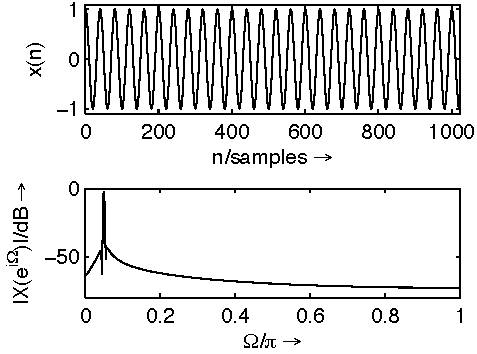
\includegraphics[scale=0.8]{fft_plot2}}
\caption{\label{fft_plot}{\it Sinusoid in time and frequency domain.}}
\end{figure}
Vectorial figures are preferred. For example when using
\texttt{Matlab}, export using either Postscript or PDF format. Also,
in order to provide a better readability, figure text font size
should be at list identical to footnote font size. To do so using
\texttt{Matlab}, use the \texttt{subplot} command before plotting.
If bitmap figures are used, please make sure that the resolution is
enough for print quality. Fig. \ref{ftt_plot2} illustrates an
example of a figure spanning two columns.
\begin{figure*}[ht]
\centerline{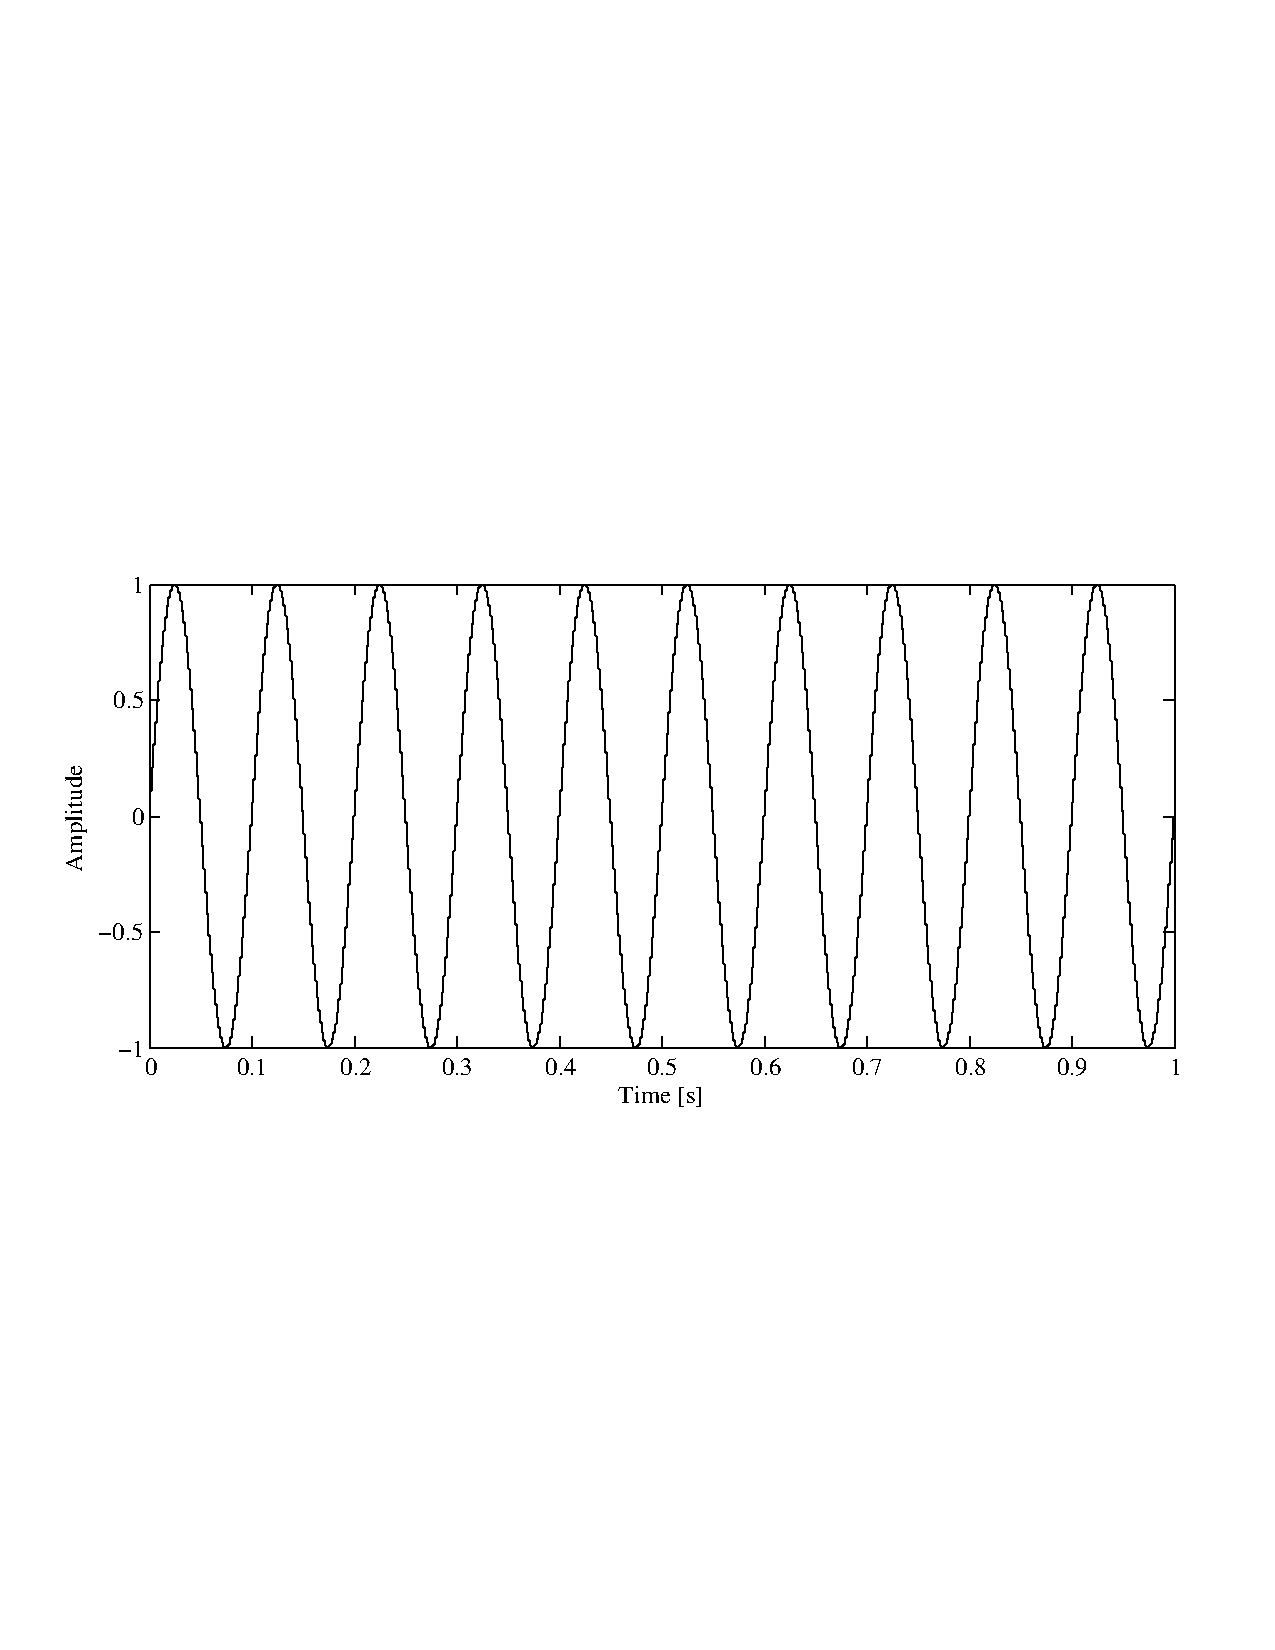
\includegraphics[width=5in,bb= 3 257 607 534]{TwoColumnSine2}} % The bounding box is set manually in this example. Useful for some .pdf figures.
\caption{\label{ftt_plot2}{\it A figure spanning two columns, as mentioned in Sec. \ref{ssec:figures}. }}
\end{figure*} % [width=5in,bb= 36 253 574 500]



%%%%%%%%%%%%%%%%%%%%%%%%%%%%%%%%%%%%%%%%%%%%%%%%%%%%%%%%%%%%%%%%%%%%%%%%%%%%%%%%%%%%%%%%%%%

\section{Conclusions}
We rock.


%%%%%%%%%%%%%%%%%%%%%%%%%%%%%%%%%%%%%%%%%%%%%%%%%%%%%%%%%%%%%%%%%%%%%%%%%%%%%%%%%%%%%%%%%%%

\section{Acknowledgments}
Thanks!


%%%%%%%%%%%%%%%%%%%%%%%%%%%%%%%%%%%%%%%%%%%%%%%%%%%%%%%%%%%%%%%%%%%%%%%%%%%%%%%%%%%%%%%%%%%

\bibliographystyle{IEEEbib}
\bibliography{../../Shared/bibtex/Jamoma} % requires file template.bib

\end{document}
